\documentclass{article}
\usepackage[utf8]{inputenc}

\title{RNN Advancements}
\author{Vinay Bhaip}
\date{April 2018}

\usepackage{natbib}
\usepackage{graphicx}
\usepackage{float}

\usepackage [english]{babel}
\usepackage [autostyle, english = american]{csquotes}
\MakeOuterQuote{"}

\usepackage{hyperref}
\hypersetup{
    colorlinks=false,
    linkcolor=blue,
    filecolor=magenta,      
    urlcolor=cyan,
}
\begin{document}

\maketitle

\section{Introduction}
Recurrent Neural Networks, or RNNs, are a type of neural network that uses sequential data within its model. RNNs aren't a new topic; they've been around since the 1980s. But with more data and computational power, they've been relevant in the fields of natural language processing, image generation, and image captioning.

\section{RNNs Review}

The main purpose of an RNN is to handle sequential data, so accordingly it should use the previous states that it outputs. In order to account for the sequential data, the RNN structure looks like this:


\begin{figure}[H]
\centering
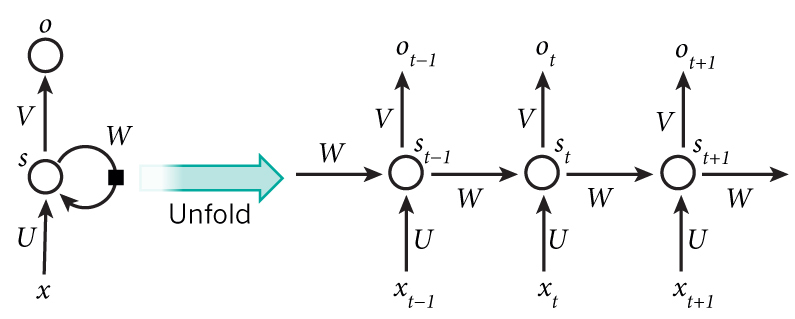
\includegraphics[scale=0.4]{basic_rnn.jpg}
\caption{A standard RNN}
\label{fig:basic_rnn}
\end{figure}

What makes an RNN different from standard networks is that the previous hidden state from the last input is passed into the function for the current state. For example, with the sentence "I like dogs", the word "I" is passed through the network and results in some output like normal. The previous hidden state that was computed for "I" is passed into the function to calculate the hidden state for "like", and so forth. This can be modeled with the equation:

\begin{equation}
    s_{t} = f(Ws_{t-1},Ux_{t})
\end{equation}

where $W$ and $U$ are weight matrices, $s_{t}$ is the state, $s_{t-1}$ is the previous state, and $x_{t}$ is the input vector. The function that the two parameters are passed into is an activation function like ReLU or tanh.

The output for each input is given through the function:

\begin{equation}
    o_{t} = g(Vs_{t})
\end{equation}

where $V$ is a weight matrix and the function is another activation function for classification, like softmax. All the weight matrices, $W$, $U$, and $V$, are the same for each layer because we basically perform the same operation at each step. Another important thing to notice is that although we can produce an output at each stage, we can choose to only use the ones we want. This comes to be helpful in scenarios like sentiment analysis where we want to model a many inputs to one output scenario.

\subsection{Backpropagation}
Backpropagation in RNNs are similar to neural networks, involving the chain rule as it takes a step back in time. If you want to see the full math behind it, check out the other RNN lecture. A problem arises in normal backpropagation when we consider our loss function:

\begin{equation}
    Loss(y,\hat{y}) = \sum_{i=0}^{t}{E_{i}}
\end{equation}

In order to calculate the loss, we would have to find the loss by propagating through the entire RNN and summing all of those errors for every single gradient step. For really long RNNs, like training on the entirety of Wikipedia, this can take a long time. This inspires the idea of \textit{truncated backpropagation through time}.

\begin{figure}[H]
\centering
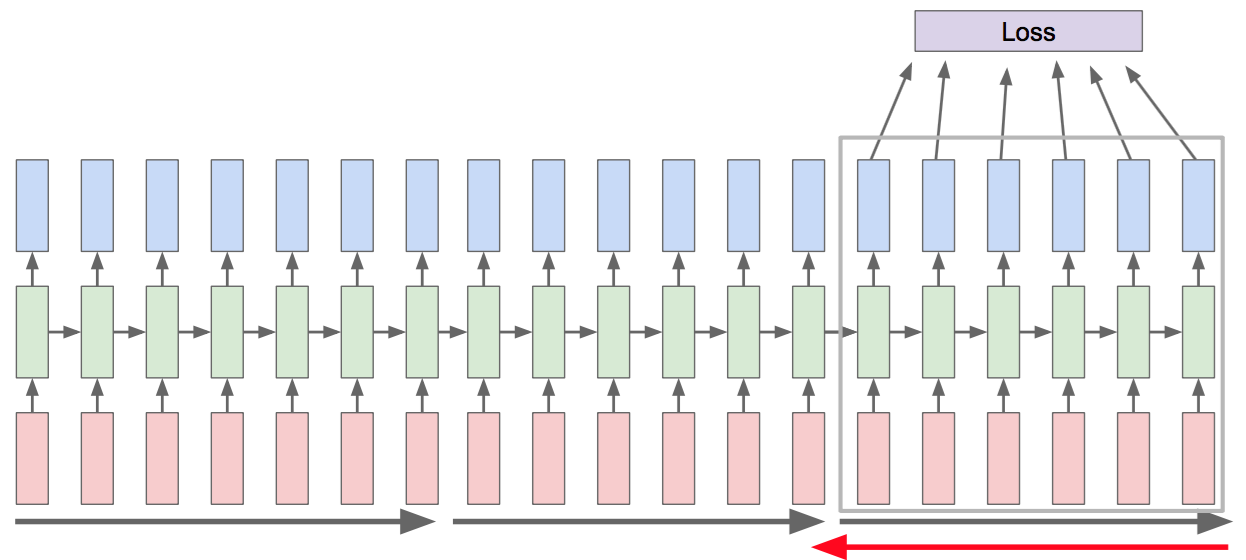
\includegraphics[scale=0.25]{truncated_backprop.png}
\caption{Truncated Backpropagation Through Time}
\label{fig:truncated_backprop}
\end{figure}

Rather than propagating and then backpropagating on the entire network, we handle it in chunks. After calculating the loss for the subset of the network that we're working with, we update the weights accordingly. A good way of thinking of this is like mini-batch; the data is taken in chunks and allows the model to converge more quickly.


\subsection{LSTMs}
Our original RNN cell looked like this: 

\begin{figure}[H]
\centering
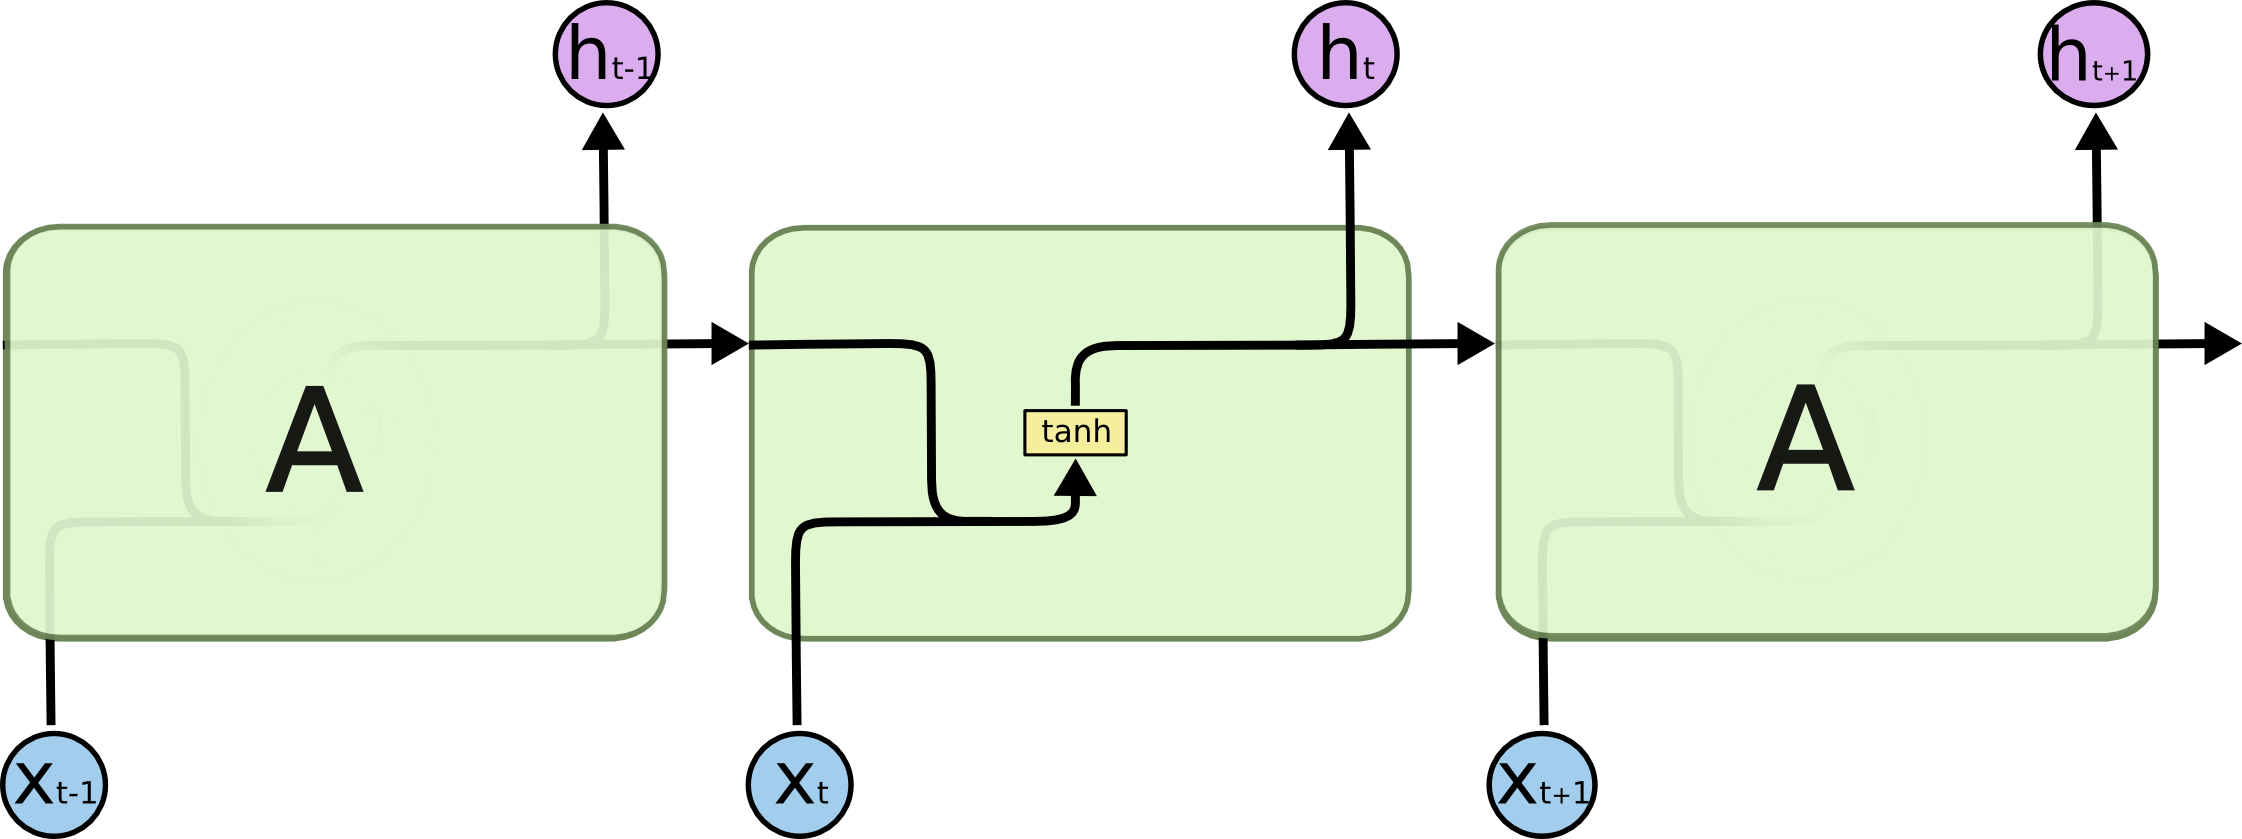
\includegraphics[scale=0.4]{lstm/rnn_basic_cell.png}
\caption{Original RNN Cell}
\label{fig:rnn_basic_cell}
\end{figure}

Notice how only the input and the hidden state are controlling the outputs of the cell.

Unfortunately, in practice, RNNs are susceptible to the vanishing gradient and the exploding gradient problem. Essentially, through backpropagation, earlier layers either face an exponentially small gradient or large gradient. This means that in sequences of data, at the current time \textit{t}, the RNN is likely to forget relevant data from long before. 

An LSTM, or Long-short term memory network, seeks to solve these problems. There are four main parts to an LSTM: the cell state ($c_{t}$), the input gate ($i_{t}$), the forget gate ($f_{t}$), and the output gate ($o_{t}$).

\begin{figure}[H]
\centering
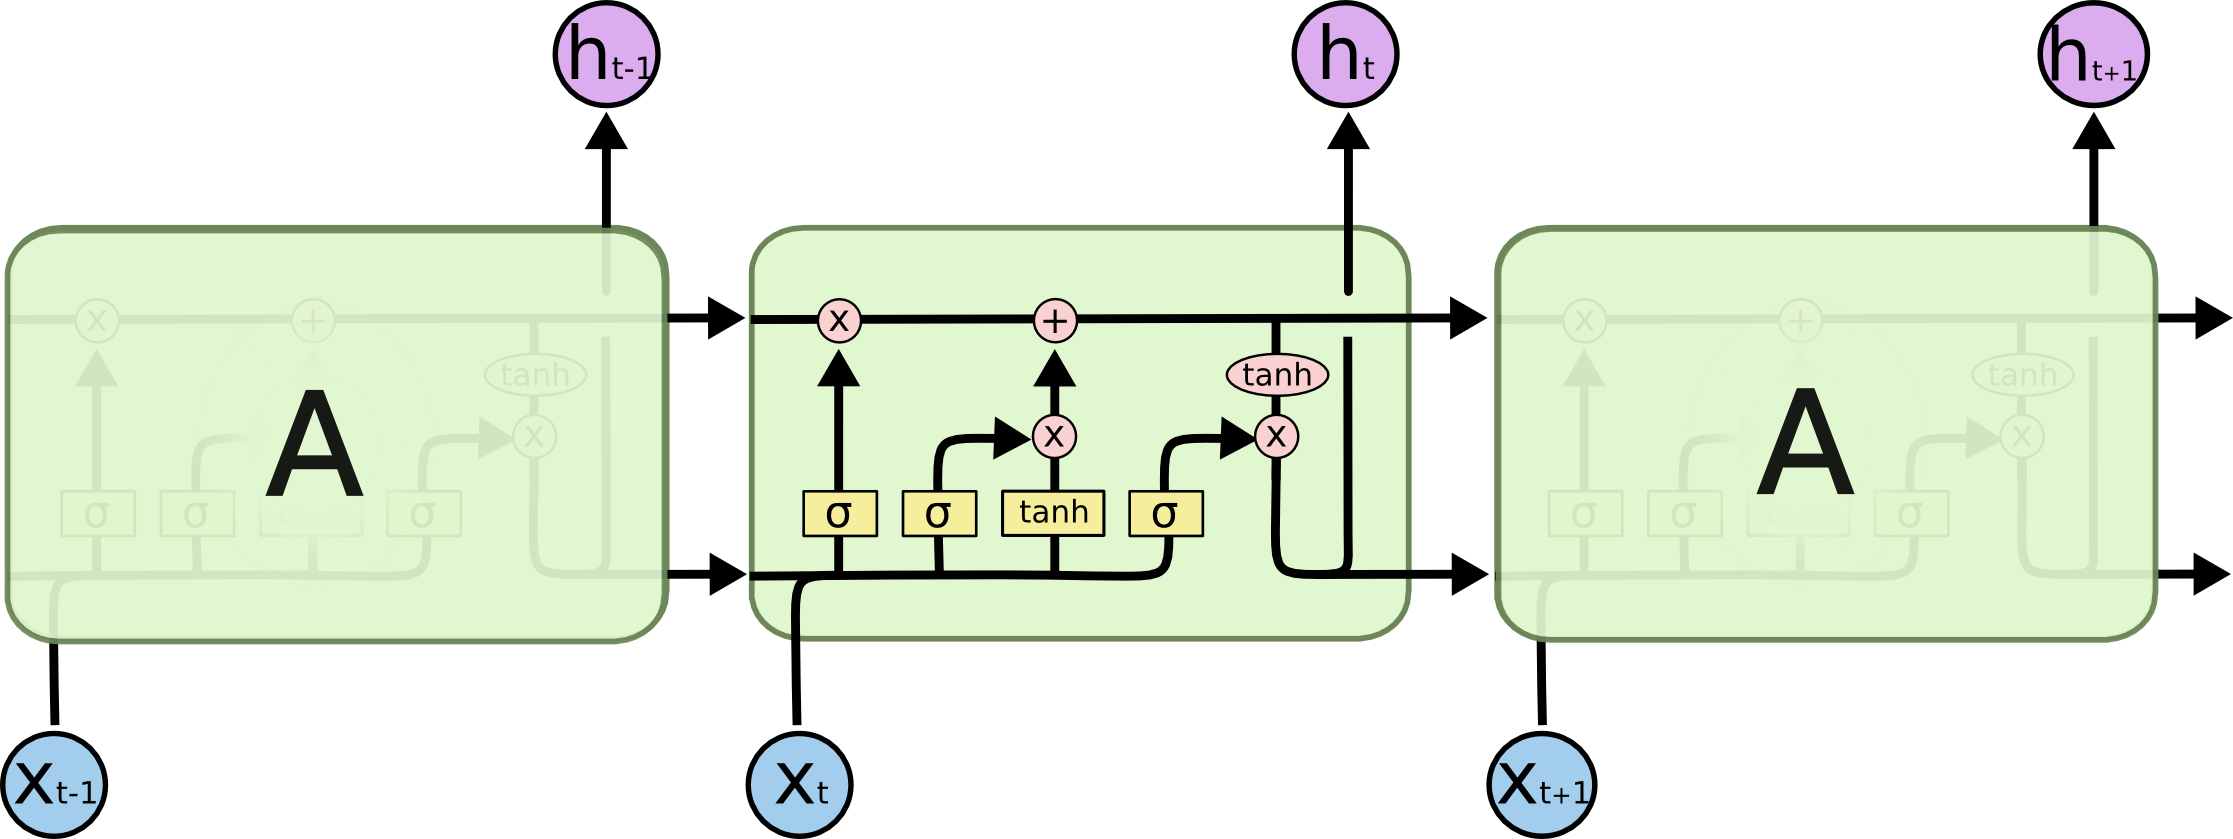
\includegraphics[scale=0.4]{lstm/lstm_main.png}
\caption{Overview of an LSTM Cell}
\label{fig:lstm_main}
\end{figure}


This cell looks a lot more complicated than the vanilla RNN we saw before. However, these added aspects improve the RNN by a lot so lets walk through them.

\begin{figure}[H]
\centering
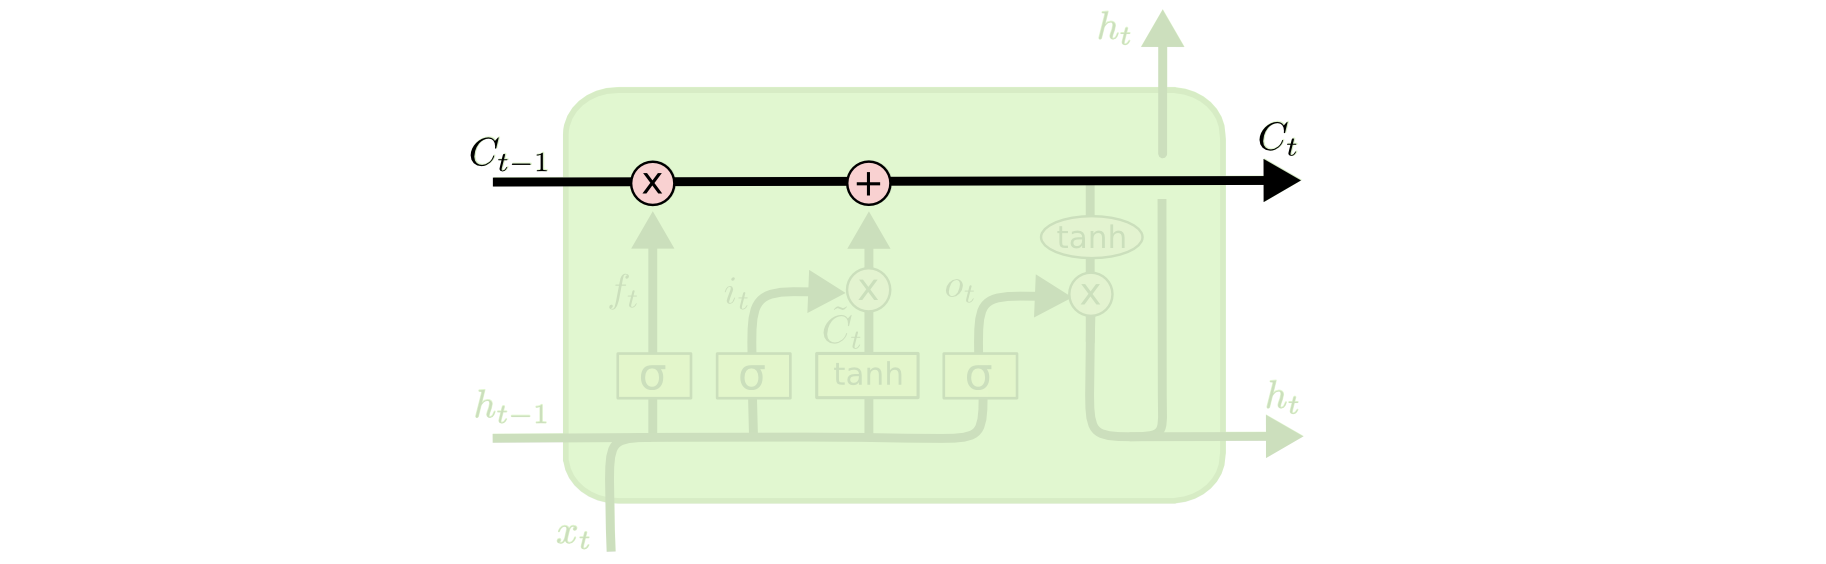
\includegraphics[scale=0.5]{lstm/lstm_cellstate.png}
\caption{LSTM Cell State}
\label{fig:lstm_cellstate}
\end{figure}

The cell state serves as the main flow across the cells. The gates modify the information that is passed through the cell state. Note, the $X$ denotes element-wise multiplication (also known as the Hadamard product) and the $+$ denotes element-wise addition.


\begin{figure}[H]
\centering
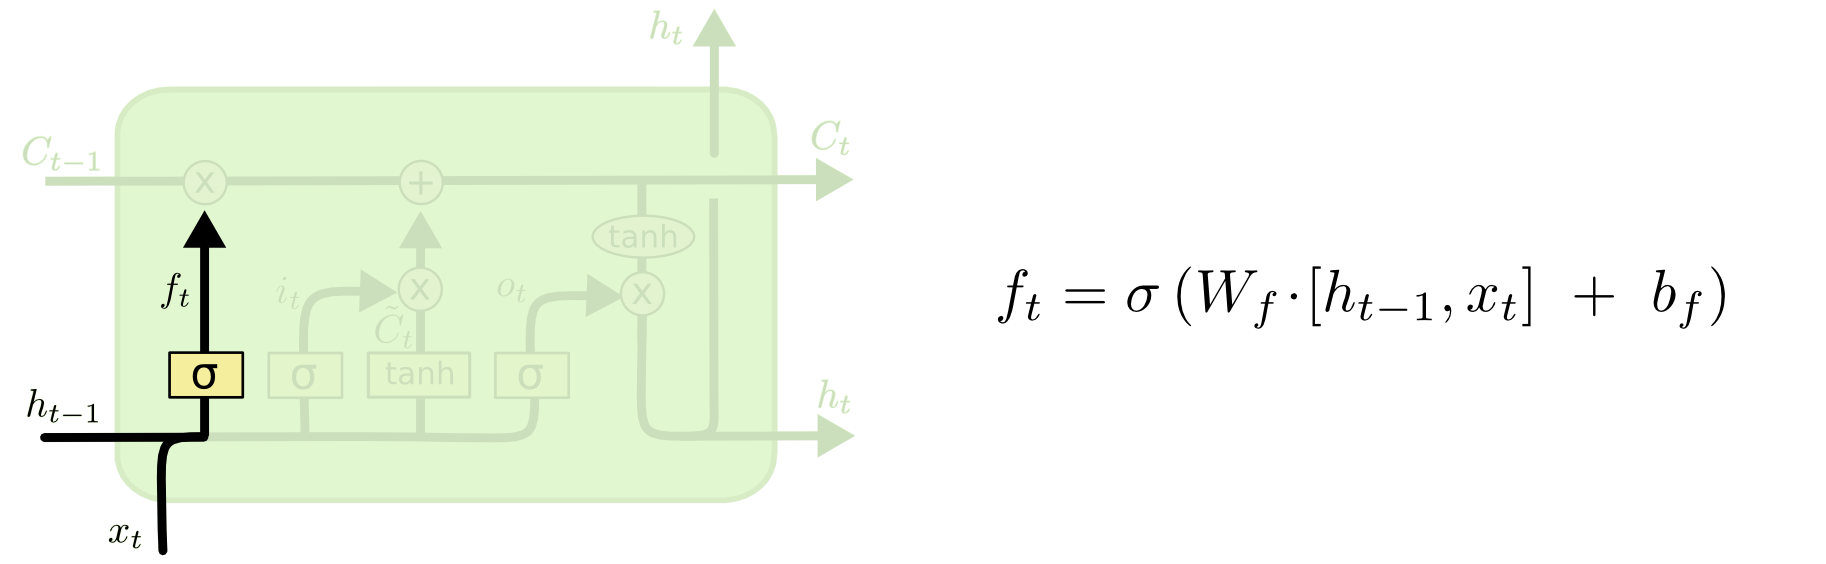
\includegraphics[scale=0.5]{lstm/lstm_forget.png}
\caption{LSTM Forget Gate}
\label{fig:lstm_forget}
\end{figure}

The forget gate chooses whether or not the information should be added to the cell state. This gate is a sigmoid layer that takes in $h_{t-1}$ and $x_{t}$. This forget gate output will be multiplied into the cell state, so if the forget gate has values of 0, then it would forget the information and if it has values of 1, then it would remember all the information.

\begin{figure}[H]
\centering
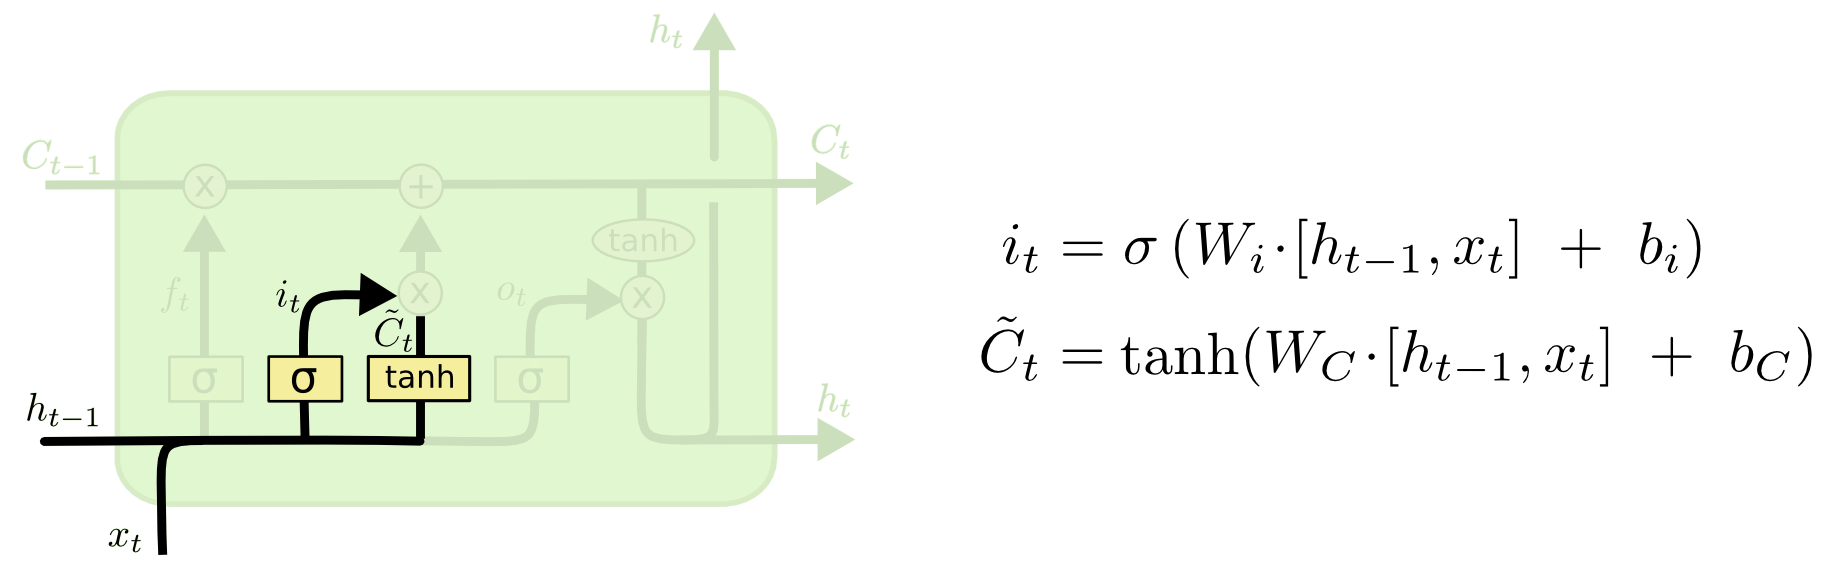
\includegraphics[scale=0.5]{lstm/lstm_input.png}
\caption{LSTM Input Gate}
\label{fig:lstm_input}
\end{figure}

Next is the input gate. This passes the input from the $h_{t-1}$ and $x_{t}$ values and combines it with the $\tilde{C}_{t}$, or new candidate values. $\tilde{C}_{t}$ takes in the inputs and looks to find new values that are possible. Notice that this is a hyperbolic tan function, which outputs values from -1 to 1. This allows the layer to give negative correlations to a value as well.

\begin{figure}[H]
\centering
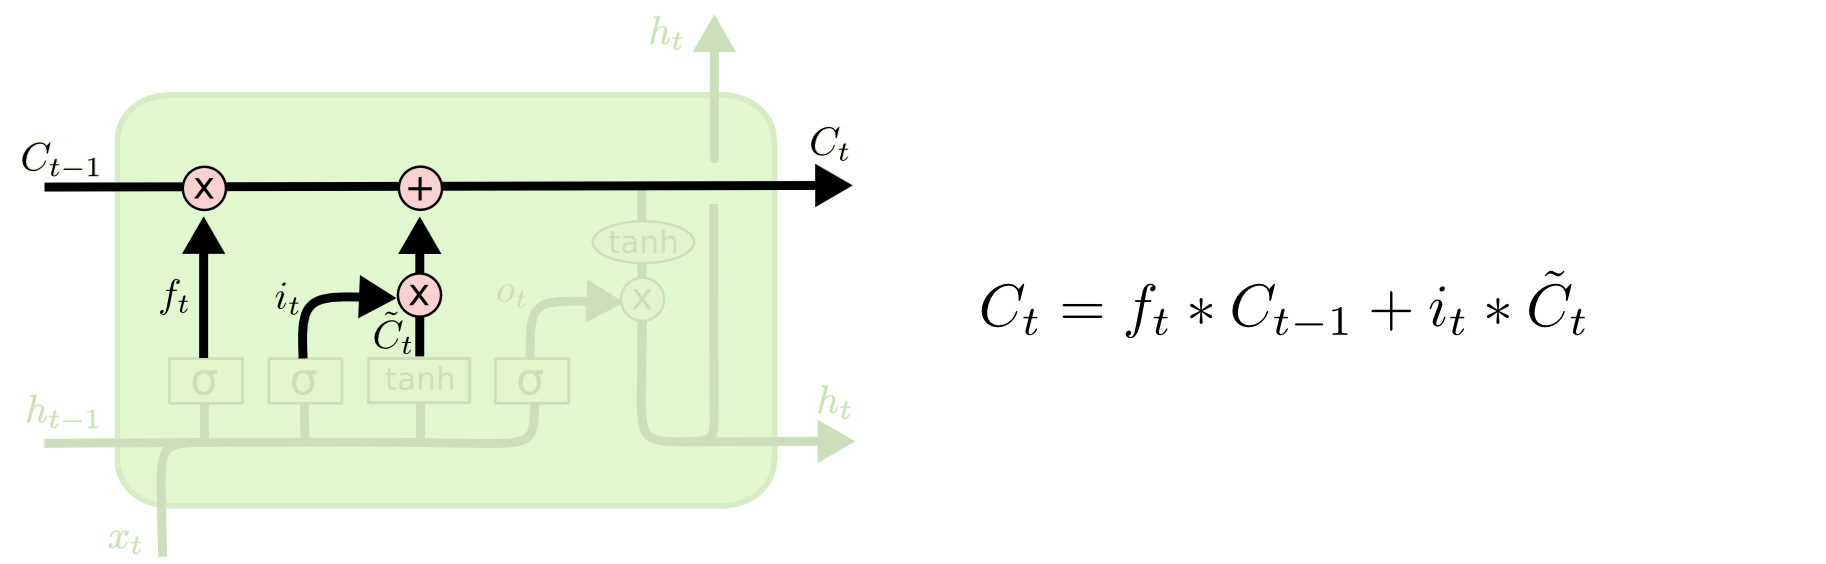
\includegraphics[scale=0.5]{lstm/lstm_combine.png}
\caption{LSTM Combining Values}
\label{fig:lstm_combine}
\end{figure}

These values are all combined and put into the cell state which passes the values through.


\begin{figure}[H]
\centering
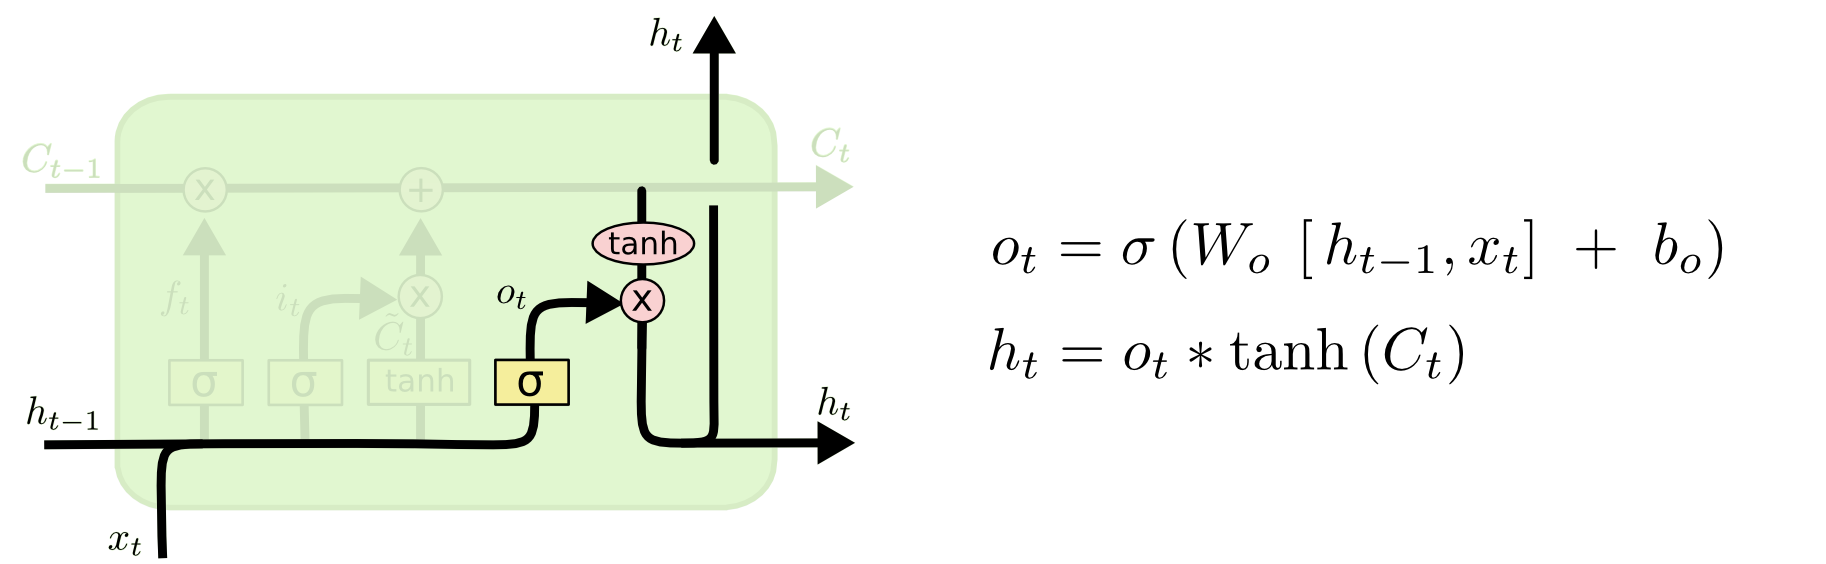
\includegraphics[scale=0.5]{lstm/lstm_output.png}
\caption{LSTM Output Gate}
\label{fig:lstm_output}
\end{figure}

Lastly, there is the output gate. This is just another sigmoid layer, which is combined with the tanh of the cell state to give the $h_{t}$ final value that gets passed into the next cell.

All these gates would be trained through backpropagation as they're just layers in a network. However, with all the layers, LSTMs can be computationally expensive, which leads us into our next section.

\subsection{GRUs}

\begin{figure}[H]
\centering
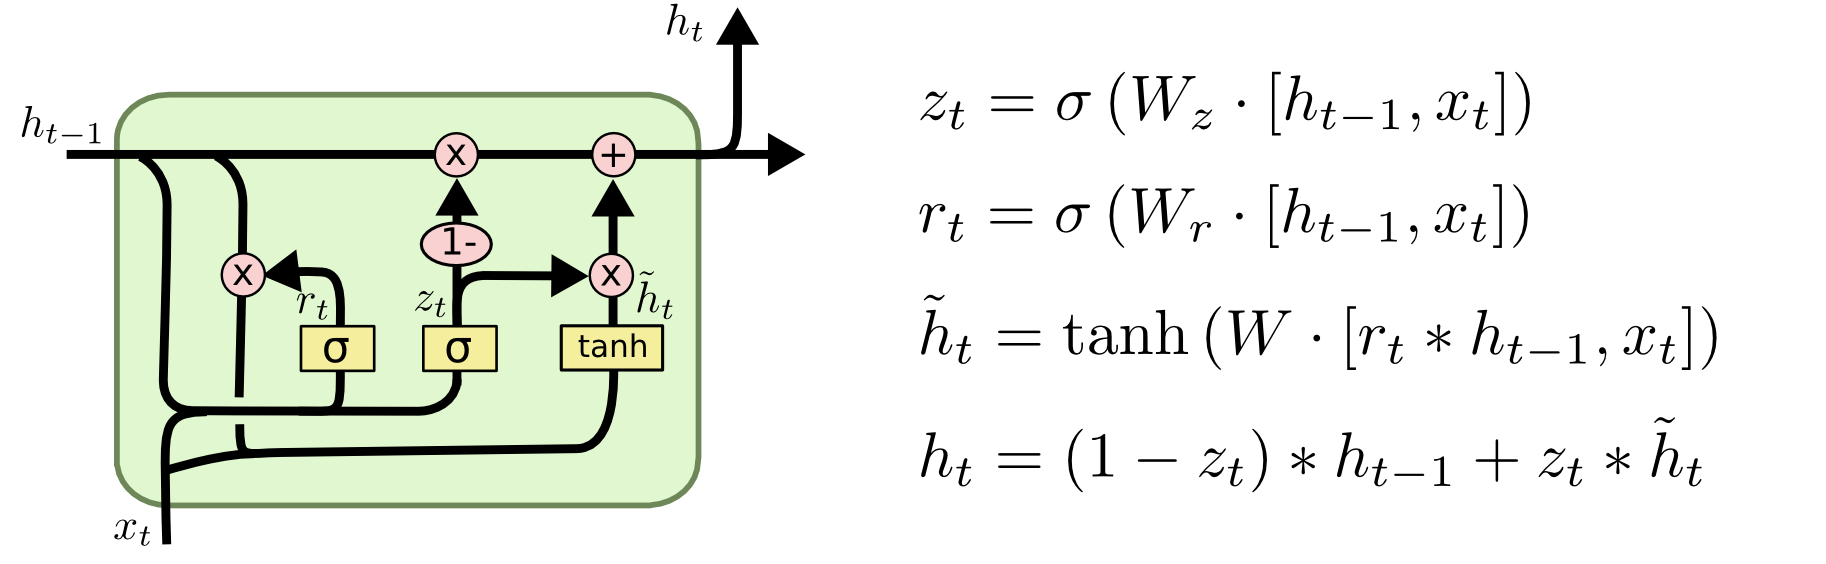
\includegraphics[scale=0.5]{GRU.png}
\caption{GRU Cell}
\label{fig:gru}
\end{figure}

GRUs, or Gated recurrent units, combine the forget and input gate into one "update" gate. Additionally, it merges the cell state and the hidden state, and adds other changes for efficiency. Fewer layers to train means a faster model.

GRUs are a relatively new concept as well, being discovered by Cho, et al. in 2014. LSTMs, on the other hand, have been around since 1997, from the discovery by Hochreiter and Schmidhuber.

\section{Language Modeling}

Now that we understand common RNNs, we can see actual applications. There are two primary ways we can model language, either character by character or word by word. For the character by character method, we would have a list of characters that are available in our vocabulary. For example, using English, we would have 26 characters plus whatever punctuation and numbers needed in our vocabulary. The same thing applies for the word by word method, but our vocabulary would comprise of all the words available.

The question then becomes how we represent this data. We can do so through \textit{one-hot encoding}. One-hot encoding means that our input vectors would be of size 1 by our vocabulary size.


\begin{figure}[H]
\centering
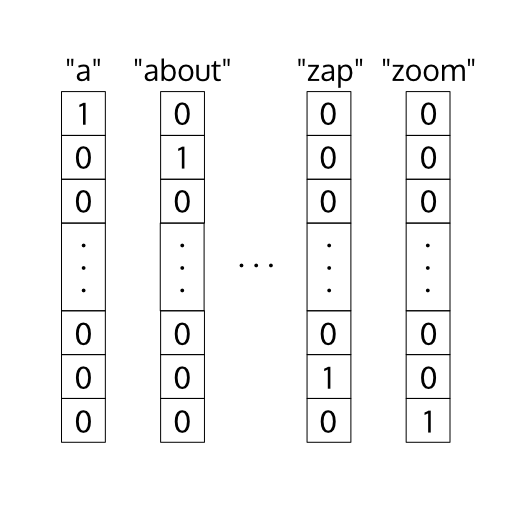
\includegraphics[scale=0.4]{one-hot-encode.png}
\caption{One-hot Encoding}
\label{fig:one-hot_encode}
\end{figure}

The reason we do this is because if we were to set each vector to be of size 1 by 1 and increment the value based on whatever is in our vocabulary, it would learn certain pieces of data to be closer than others. For example, if we had the vocabulary of [a, b, c] and set the vectors for each one respectively to be [0], [1], and [2], our model would think that "a" and "b" are closer together than "a" and "c", which obviously doesn't make sense.

Another question with RNNs becomes how can we generate new text to continuously go on. The way this works is we pass in a seed value for the $x_{0}$, or the initial value that goes in. From that we get some output from the softmax function, which we take the maximum of as our value. To continue this chain, we pass this output as the $x_{t+1}$ input vector.

For this, when we choose what to pass in as the next input vector, we can either just pass the highest value from our softmax, or alternatively, we can sample from the softmax probabilities and pass that for the next input. The reason as to why we do this is to generate multiple new types of output sequences giving more diversity to the model.

\subsection{Sequence to Sequence Models}
The goal of a sequence to sequence model is to map one sequence to another sequence. This can be done by having two RNNs, one as an \textit{encoder} and the other as a \textit{decoder}. The encoder takes in a sequence and maps it to one output vector and the decoder takes that one output vector and maps it to another sequence. In other words, an encoder is in the format of a many to one structure and the decoder is in the format of a one to many structure.

\begin{figure}[H]
\centering
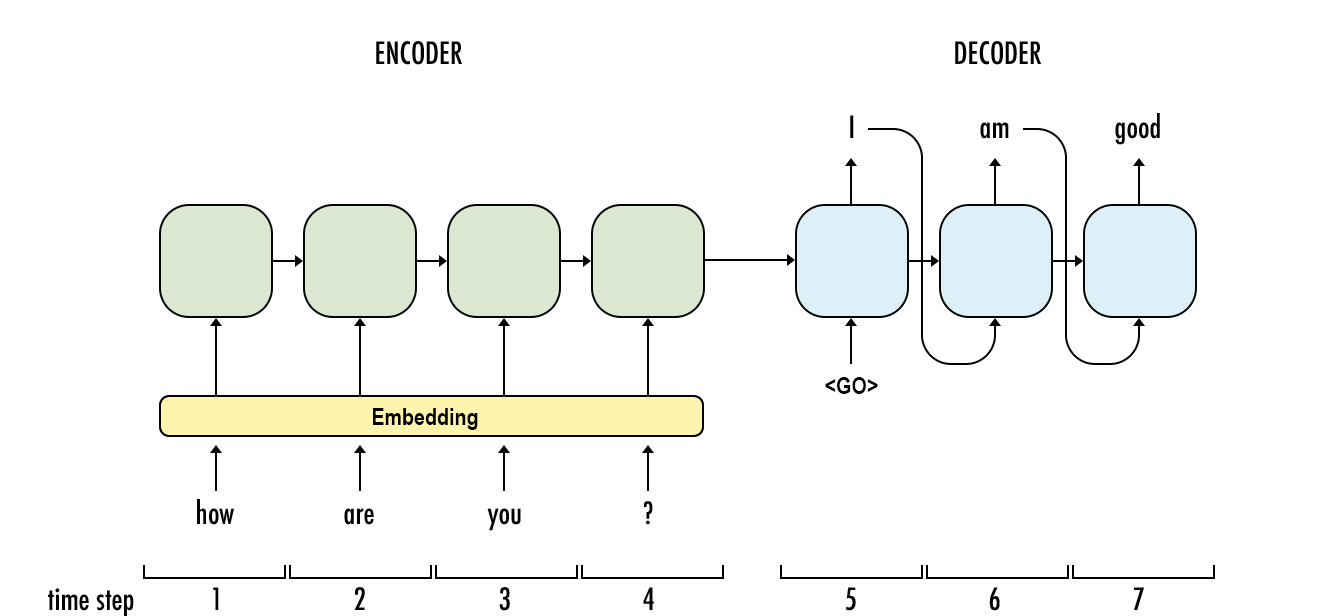
\includegraphics[scale=0.2]{seq2seq.png}
\caption{A Seq2Seq Model}
\label{fig:seq2seq}
\end{figure}

In the figure above, we can see that this model can be used for chat bots and also for machine translation, meaning we take words of one language and convert them into words of another language.

How does the model know when to stop translating? In training, there would be an end of sequence token appended onto the end of the translated text, like $<EOS>$, which signifies that the translation should stop.

\subsection{Autoencoders}
An autoencoder attempts to compress a vast amount of information into one dense object, without losing any of the information. The middle part of an autoencoder is the compressed version of the data.


\begin{figure}[H]
\centering
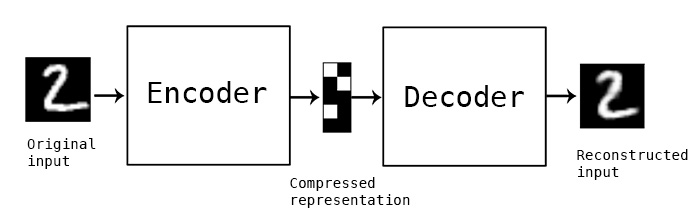
\includegraphics[scale=1.8]{autoencoder.jpg}
\caption{An Autoencoder}
\label{fig:autoencoder}
\end{figure}

When coding this model, in Keras for example, everything is done the same as if making a standard model, but we run $Model.fit(X,X)$ instead of $Model.fit(X,Y)$. This is so the model can map the same value to itself, while compressing it inside the image.

The reason this can prove to be useful in Seq2Seq models is because when in the task of machine translation, the middle part represents a universal part of the text. So when translating between English and German, the RNN could encode the data into one vector with the information, and pass that to a decoder to translate the original text.

\subsection{Attention}

As great as sequence to sequence models are, we are relying on the last token of the encoder to contain all the information for the entire output sequence. Each part of the input sequence should play a different role for each part of the output sequences. 

\begin{figure}[H]
\centering
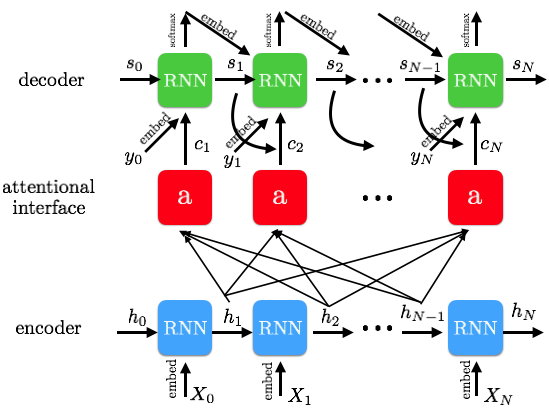
\includegraphics[scale=.5]{attention_rnn.png}
\caption{Attentional RNN}
\label{fig:attention_rnn}
\end{figure}

Into each RNN cell, we pass in a weighted combination of the input states, which allows each output result to attend to different parts of the input sequence. This concept, accordingly so, is called \textit{attention}. For each state of the decoder at a time step, $s_{t}$, the sum of each weight multiplied by its respective input hidden state is added. In other words, the attention added for each state \textit{i} is generally in the structure:

\begin{equation}
a = \sum_{i=1}^{t}a_{i,t}*h_{i}
\end{equation}

Visualizing the weight matrix $a$ lets us see what input words contribute to each output word:


\begin{figure}[H]
\centering
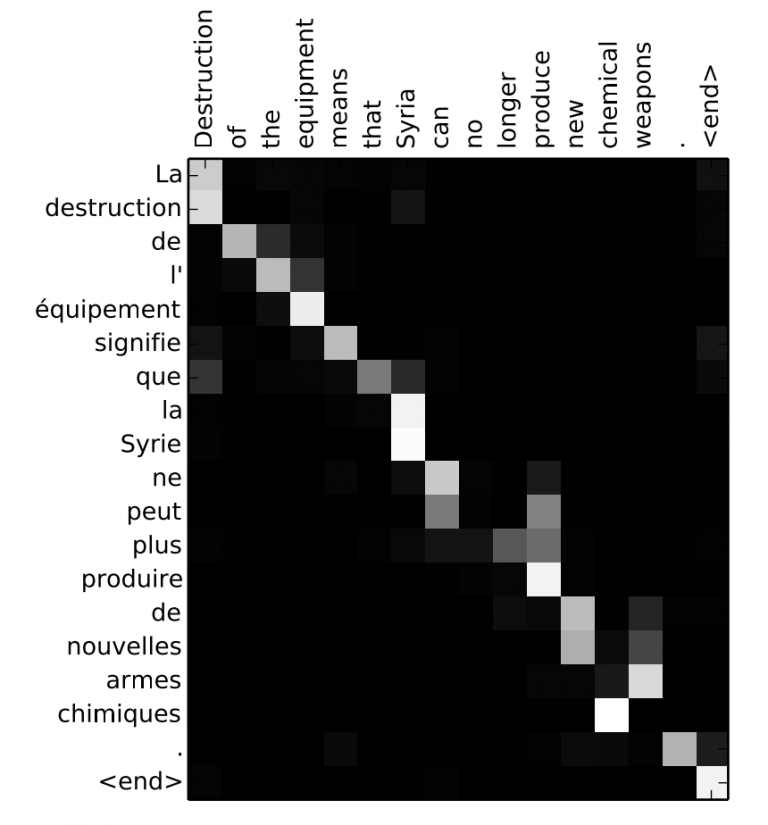
\includegraphics[scale=.3]{attention_example.png}
\caption{Attention Visualized}
\label{fig:attention_example}
\end{figure}

In this visualization of a translation of a French sequence to an English sequence, the squares that are brighter show where the attention is activated. For example, the first box on the top left shows that "La" contributes to the output of "Destruction". The overarching trend shows that the model goes through the inputs in order for the most part when generating the output. However, we can see attention really working in examples like when both the inputs "la" and "Syrie" contribute to the output term "Syria".

An important concept in attention is this idea of \textit{hard attention} versus \textit{soft attention}. Hard attention focuses on one fixed area of the input, whereas soft attention takes in a weighted distribution of where to look.

\begin{figure}[H]
\centering
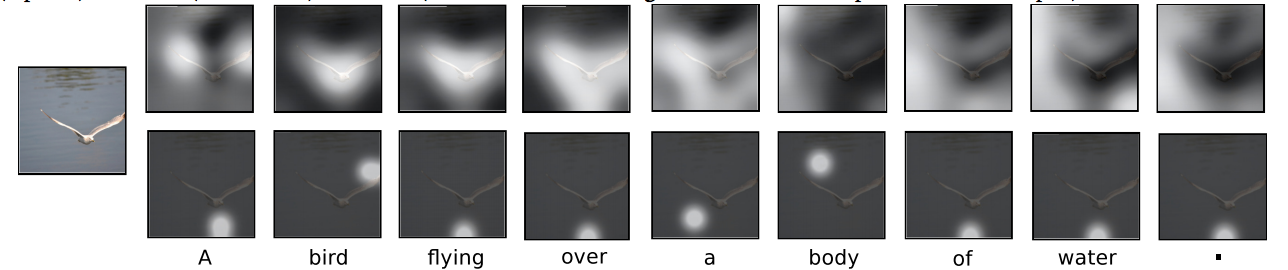
\includegraphics[scale=.5]{softvhard_attention.png}
\caption{Soft vs. Hard Attention}
\label{fig:softvhard_attention}
\end{figure}

Notice how in the top row of images, each image shows a distribution of the regions that are being looked at but in the bottom row images, each image shows a direct location that is being looked at. The problem with hard attention is that it isn't differentiable, so different techniques have to be applied to work around that. 

Even though attention seems to be really helpful, when the input sizes and the output sizes increase, the amount of values for attention needed increases by a lot as well. This can also be inefficient for long character by character models. A possible solution for this is using reinforcement learning to filter out areas where the attention isn't needed.


\section{PixelRNN}

A cool application of RNNs is for filling in areas of an occluded image. The interesting part of the paper which this concept was the introduction of a 2D RNN.

The two main techniques employed were the Row LSTM and the Diagonal BiLSTM. This lecture won't get into the specifics of how each was used, but the general concept was that the Row LSTM went pixel by pixel horizontally, and the Diagonal BiLSTM accordingly goes pixel by pixel on the diagonals, with a convolution kernel size of 2.

\begin{figure}[H]
\centering
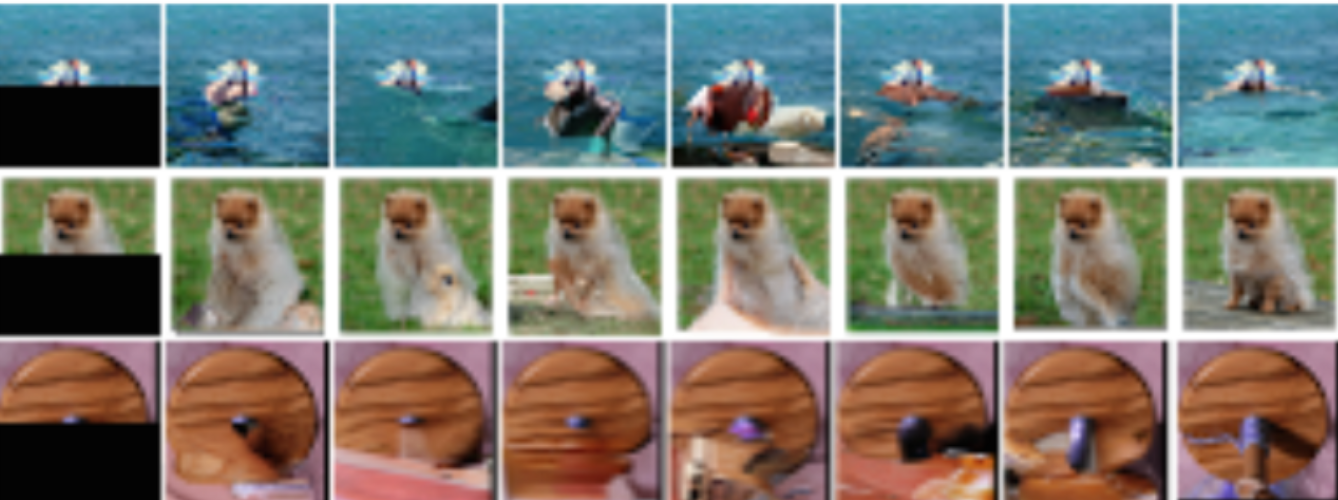
\includegraphics[scale=.225]{pixelrnn.png}
\caption{PixelRNN Outputs}
\label{fig:pixelrnn}
\end{figure}

On the left are the images that would be passed in, with the occlusion, and on the right are the ground truth images. All the images in between are the generation by the network. From some distance away, it sortof looks accurate, but close-up, the images are obviously not perfect.

\section{DRAW Network}

DRAW, or the Deep Recurrent Attentive Writer, is an RNN for image generation, but does so in a way that tries to mimic the way humans create images.

\begin{figure}[H]
\centering
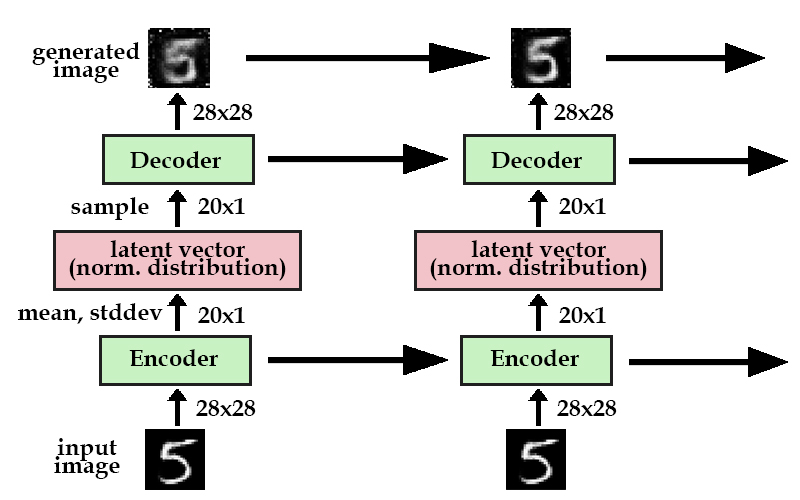
\includegraphics[scale=.35]{draw_structure.jpg}
\caption{DRAW Model}
\label{fig:draw_structure}
\end{figure}

Although this seems like an autoencoder, it's actually a different type of autoencoder than mentioned earlier in the lecture. This network specifically uses a \textit{variational autoencoder} (VAE). VAEs are essentially generative autoencoders; the encoder creates a latent vector that has a probability distribution, which the decoder samples from to create the generated image. Why go through this? This makes sure that different images can be generated through the same input image, because the model learns the underlying distribution.

Now we have an RNN that can sequentially make the generated image over time. But looking at the sequence of generated images at each time step, the model is drawing on the entire image and making small changes each time. We would rather have the model work in one area and move around as if it was actually drawing it by hand. This is where attention comes in.

\begin{figure}[H]
\centering
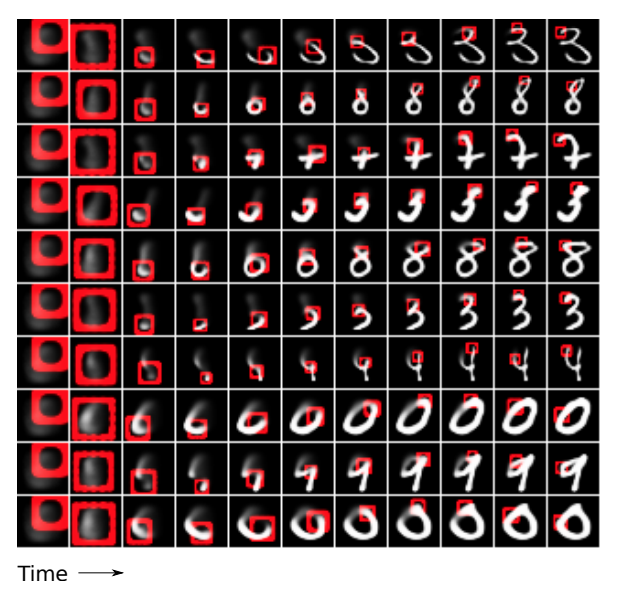
\includegraphics[scale=.7]{draw_attention.png}
\caption{DRAW with Attention}
\label{fig:draw_attention}
\end{figure}

To keep things simple, basically there's an added attention gate, which tells the model where to focus on. This continuously shifts at each time step, until the model finishes the image. The end result of these images is pretty successful.

\begin{figure}[H]
\centering
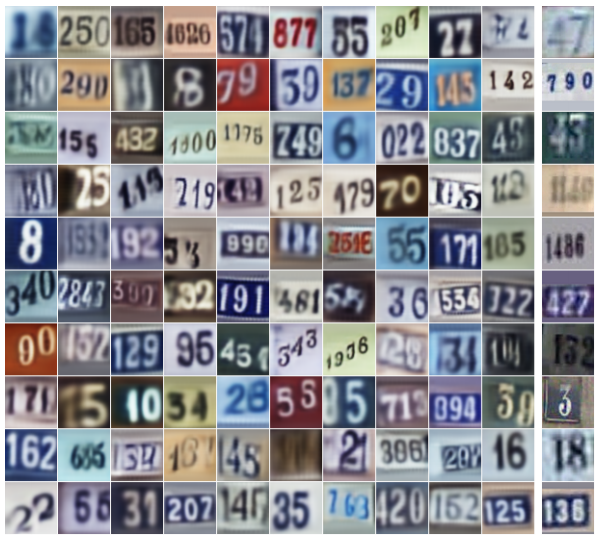
\includegraphics[scale=.7]{draw_streetview.png}
\caption{DRAW Generated Street View House Numbers}
\label{fig:draw_streetview}
\end{figure}

These generated images of house numbers looks really accurate, and basically indistinguishable from real pictures of house numbers.

\section{Conclusion}
There's a lot within the field of RNNs, and is growing rapidly as it sees applications all over. This lecture should have given you a glimpse into RNNs and the advancements that are currently happening.

\section{Acknowledgements}

I did not create any diagrams or images in this lecture. All credits go to their respective owners. Here are most of the sources I used:

\begin{itemize}
    \item \href{http://www.youtube.com/watch?v=6niqTuYFZLQ}{Stanford RNN CS231n Lecture}
    
    \item \href{http://colah.github.io/posts/2015-08-Understanding-LSTMs/}{Christopher Olah's LSTM Walkthrough}
    
    \item \href{https://arxiv.org/pdf/1601.06759v2.pdf}{PixelRNN Paper}
    
    \item \href{https://arxiv.org/pdf/1502.03044.pdf}{Attention Paper}
    
    \item \href{https://arxiv.org/pdf/1502.04623.pdf}{DRAW Paper}
    
    \item \href{http://kvfrans.com/what-is-draw-deep-recurrent-attentive-writer/}{Kevin Fran's DRAW Walkthrough}

\end{itemize}

\end{document}
